% \documentclass[12pt,a4paper,openany, ]{book} %el comando "openany" sirve que cuando se hace un Chapter, dejará una hoja en blanco.
\documentclass[12pt,letterpaper]{book}
\usepackage[ruled,vlined]{algorithm2e}
\usepackage{tabularx}
\usepackage{longtable}
\usepackage[utf8]{inputenc}
\usepackage[T1]{fontenc}

\usepackage{tgtermes} % times font

\usepackage[spanish,es-tabla]{babel}
\usepackage{amsmath}
\usepackage{amsfonts}
\usepackage{amssymb}
\usepackage{graphicx}
\usepackage{subfig}
\usepackage{wasysym}
\usepackage{lscape}
\usepackage[colorlinks=true, linkcolor=black,
citecolor=black, urlcolor=black,hidelinks]{hyperref}
\usepackage{float}
\usepackage{booktabs}
\usepackage{setspace} %por si el titulo es mas largo y el interlineado
\usepackage{xcolor} %para darle color a las lineas del titulo.
\usepackage{lipsum} %crea texto ficticio del texto Lorem Ipsum
%\definecolor{azul}{rgb}{0.17, 0.4, 0.69} %definir color de lineas.
% \usepackage{natbib}
%\usepackage[left=2.54cm,top=2.54cm,right=2.54cm,,bottom=2.54cm]{geometry} %para cambiar la configuracion de las medidas a APA se usa "Control + R".

\usepackage[left=3cm,top=3cm,right=3cm,,bottom=4cm]{geometry}

\usepackage[justification=centering]{caption}
% Reducimos el espacio debajo de las figuras
\captionsetup{belowskip=0pt}

\newcommand{\grad}{$^{\circ}$}
\renewcommand{\baselinestretch}{1.5} %interlineado 1.5

\usepackage{csquotes}
\usepackage[backend=biber,natbib,url=false,doi=false,style=apa,maxcitenames=5]{biblatex}

% Cuando el idioma es otro "et al." cambia, con este comando se fuerza a si o si usar "et al."
\DefineBibliographyStrings{spanish}{%
  andothers = {et\addabbrvspace al\adddot}
}
% \addbibresource{capitulos/biblio.bib}

\renewcommand{\labelenumii}{\arabic{enumi}.\arabic{enumii}}
\renewcommand{\labelenumiii}{\arabic{enumi}.\arabic{enumii}.\arabic{enumiii}}
\renewcommand{\labelenumiv}{\arabic{enumi}.\arabic{enumii}.\arabic{enumiii}.\arabic{enumiv}}

% SE ELIMINA LA PALABRA "CAPÍTULO" DEL TÍTULO
\usepackage{titlesec}

% Capítulos sin la palabra "Capítulo "
\titleformat{\chapter}
  {\normalsize\bfseries}{\thechapter.}{0.5em}{}
%   \titlespacing*{\chapter}{0pt}{2pt}{2pt}
\titlespacing*{\chapter}{0pt}{0pt}{0pt}[0pt]
% \titlespacing*{\chapter}{0pt}{3.5ex plus 1ex minus .2ex}{2.3ex plus .2ex}

% Cambiamos el tamaño de las secciones
\titleformat{\section}
  {\normalfont\normalsize\bfseries}{\thesection.}{0.5em}{}
\titleformat{\subsection}
  {\normalfont\normalsize\bfseries}{\thesubsection.}{0.5em}{}

% SE ELIMINA LA CABECERA DE LAS HOJAS Y LA NUMERACIÓN ES ABAJO
\usepackage{fancyhdr}
\fancyhf{}
\renewcommand\headrulewidth{0pt}
% \fancyfoot[RO, LE]{\thepage}
% \fancyfoot[C]{\thepage}
% SE ENUMERA A LA DERECHA
\fancyfoot[R]{\thepage}
% SE REDEFINE EL ESTILO PARA ENUMERAR LAS PÁGINAS DE CAPÍTULO A LA DERECHA
\pagestyle{fancy}
\fancypagestyle{plain}{%
    \renewcommand{\headrulewidth}{0pt}%
    \fancyhf{}%
    \fancyfoot[R]{\thepage}%
}

% \renewcommand{\contentsname}{Índice}

\usepackage[subfigure]{tocloft}
% \setlength{\cftpartindent}{0em}
% \setlength{\cftchapindent}{0em}
\setlength{\cftsecindent}{0em}
\setlength{\cftsubsecindent}{0em}
\setlength{\cftsubsubsecindent}{0em}
% \setlength{\cftsubsubsecindent}{3em}

\usepackage{enumitem}
\setcounter{tocdepth}{4}
\setcounter{secnumdepth}{4}

\renewcommand*{\listalgorithmcfname}{Lista de Algoritmos}
\renewcommand*{\algorithmcfname}{Algoritmo}
\renewcommand*{\algorithmautorefname}{algoritmo}
\SetKwInput{KwData}{Requiere}

\makeatletter
\patchcmd{\chapter}{\if@openright\cleardoublepage\else\clearpage\fi}{}{}{}
\makeatother

% Contar las figuras sin el capítulo
\usepackage{chngcntr}
\counterwithout{figure}{chapter}

% Editando el titulo del indice
\addto\captionsspanish{% Replace "spanish" with the language you use
  \renewcommand{\contentsname}%
    {\fontsize{16}{20}\selectfont ÍNDICE}
}
% quitando espacio del titulo del indice
\setlength{\cftbeforetoctitleskip}{-1em}
\setlength{\cftaftertoctitleskip}{1em}

% Quitando el identado en cada parrafo
\setlength\parindent{0pt}

% Espaciado entre parrafos
\setlength{\parskip}{0.5em}

\begin{document}
	%FRONTMATTER
	%---------------------------------------------------
	\frontmatter %numeros romanos
	\newgeometry{top=2.5cm, bottom=2.5cm, left=2.5cm, right=2.5cm}
\begin{titlepage} %este titlepage sirve para poder realizar el titulo de una pagina, la caratula de un libro y no se enumere esta.
	\begin{center}
	    {\fontsize{20}{20}\selectfont \textbf{UNIVERSIDAD MAYOR DE SAN ANDRÉS}}\\
		{\fontsize{16}{16}\selectfont \textbf{FACULTAD DE CIENCIAS PURAS Y NATURALES\\
		CARRERA DE INFORMÁTICA}}
		%\vspace{1mm}
		
		% 
\includegraphics[height=8cm]{images/logo_umsa.png}
		
\includegraphics[scale=0.20]{images/logo_umsa.png}
		%\vspace{1mm}
		
		{\fontsize{16}{20}\selectfont \textbf{TESIS DE GRADO}}\\
		%\vspace{2mm}
		
        {\fontsize{16}{18}\selectfont \textbf{COMPARACIÓN Y REFINAMIENTO DE ALGORITMOS DE FACTORIZACIÓN DE NÚMEROS ENTEROS}}
		
		{\fontsize{12}{12}\selectfont\textbf{Tesis de Grado para obtener el Título de Licenciatura en Informática Mención Ciencias de la Computación}}
 		%\vspace{2mm}
		
		{\fontsize{16}{16}\selectfont\textbf{POR: ROLANDO TROCHE VENEGAS}}\\
    	{\fontsize{14}{14}\selectfont\textbf{TUTOR: M.SC. JORGE HUMBERTO TERÁN POMIER}}
		%\vspace{2mm}
		 
		\textbf{LA PAZ - BOLIVIA\\
		2024}
	\end{center}
\end{titlepage}
\restoregeometry
% 	\include{jurado}
% 	\clearpage

% \thispagestyle{empty} 

% \vspace*{\fill} 

\begin{flushleft}
\begin{center}
  \textbf{AGRADECIMIENTOS}
\end{center}

\textit{Quiero expresar mi más sincero agradecimiento a todos aquellos que me han brindado su apoyo y guía durante la elaboración de esta tesis: }\\
A mis padres, por su incondicional apoyo a lo largo de mi carrera y por ser mi fuente constante de inspiración y motivación. \\

A mi tutor, el M. Sc. Jorge Teran Pomier, por su invaluable apoyo, confianza y orientación durante todo el proceso de elaboración de esta tesis. \\

Al Club de Programación Competitiva U.M.S.A., por todo lo aprendido y las experiencias compartidas, las cuales han enriquecido mi formación y desarrollo profesional. \\

A mis amigos, "Los Osos", por ser los mejores compañeros que pude tener y por su compañía durante todo este camino en la universidad. \\ 

Finalmente, al lector, gracias por darle vida y sentido a este trabajo con su interés y atención. \\
% A mis padres por apoyarme a lo largo de mi carrera. \\
% A mi tutor M. Sc Jorge Teran Pomier por su apoyo y confianza en el proceso de elaboración
% de la presente tesis.\\
% Al Club de Programación Competitiva U.M.S.A. por todo lo aprendido y las experiencias que tuvimos.\\
% A los Osos, por ser los mejores amigos que pude tener y acompañarme durante este camino en la universidad. \\
% Al lector, gracias por darle vida y sentido a este trabajo.
\end{flushleft}

\vspace{\fill}
\begin{flushright}
  rtrochevenegas@gmail.com
\end{flushright}
	
	%ÍNDICE O TABLA DE CONTENIDO-------------------
	\tableofcontents
	\setcounter{page}{0}
	%\cleardoublepage
% 	\addcontentsline{toc}{chapter}{Lista de figuras} % para 						que aparezca en el indice de contenidos
% 	\listoffigures % indice de figuras
	%\cleardoublepage
% 	\addcontentsline{toc}{chapter}{Lista de tablas} % para que 						aparezca en el indice de contenidos
% 	\listoftables % indice de tablas
	
	 % si no queremos que añada la palabra "Capitulo"
% 	\addcontentsline{toc}{chapter}{INTRODUCCIÓN} % si queremos que aparezca en el índice
	%\markboth{AGRADECIMIENTOS}{AGRADECIMIENTOS} % encabezado
	
	%MAINMATTER
	%--------------------------------------------------	
	\mainmatter %numeros arabicos.
    
    % \begingroup
    % \renewcommand{\cleardoublepage}{}
    % \renewcommand{\clearpage}{}
    
    \raggedbottom
    
    % \thispagestyle{empty}
    % \input{capitulos/01-introduccion}
    \chapter{INTRODUCCIÓN}

    % \section{INTRODUCCIÓN}

    \thispagestyle{empty}

    Factorizar números enteros es importante, hoy más que nunca la factorización de números enteros juega un papel crucial en la vida de todas las personas. Los métodos de encriptación actuales se basan, en gran medida, en la complejidad y el tiempo que toma factorizar números grandes.

    También se debe notar la definición de número grande, si se le pregunta a un niño que es un número grande este puede decirnos que es el 100 o hasta el 1000 y si se le preguntara a una persona adulta esta podría decirnos 1 000 000 o 100 000 000, pero esto no es nada si se piensa en los problemas que hoy en día lidian los matemáticos.

    Factorizar un número se refiere a encontrar todos los factores primos por los que está compuesto dicho número. El teorema fundamental de la aritmética nos dice que para todo número entero positivo mayor a 1 es un numero primo o bien un único producto de números primos (Euclides, 300 AC).
    \[
    n = \prod_{i=1}^{k}p_{i}^{a_{i}}
    \]
    Este es el objetivo que buscamos, encontrar esos factores para números, ahora sí, grandes.

    Los algoritmos de encriptación actuales, como RSA, usan números de, por ejemplo, 250 dígitos (829 bits) que fue el último en ser factorizado febrero de 2020. Estos son los números grandes que nos interesan. Los números RSA por ejemplo son números con exactamente dos factores primos, estos números primos, de al menos, la mitad de cantidad de dígitos que el resultado.

    Hoy en día tenemos diferentes métodos de factorización como los algoritmos simples de factorización, fracciones continuas, curva elíptica, algoritmos de cribado y hasta nuevos algoritmos basados en programación cuántica.

    En este trabajo se estudiará los diferentes métodos de factorización de números y su implementación con diferentes enfoques y refinamientos de implementación que el autor propondrá para ciertos métodos. Con esto se podrá revisar los alcances de los algoritmos de encriptación actuales y a donde se puede llegar en base a estos y realizar una comparación de los mismo, mostrando que algoritmo es el adecuado dada ciertas condiciones.
    \newpage
    % % \pagenumbering{arabic}
    % \input{capitulos/02-antecedentes}
    % \input{capitulos/03-planteamiento-del-problema}
    \chapter{PROBLEMA}
    % \section{ANTECEDENTES}
    
    \section{PLANTEAMIENTO DEL PROBLEMA}
    Con el avance de las computadoras y el mayor poder de cómputo, toda la seguridad basada en factorización y factores primos corre riesgo de quedar deprecada algún día.

    Por esto es necesario tener un compendio de gran parte de los métodos y algoritmos de factorización existentes y sus limitaciones, con el poder de cómputo actual. Por otro lado, hoy en día con la ayuda de los nuevos y mejores procesadores muchos algoritmos pueden ser paralelizados lo que reduciría su tiempo de ejecución.

    \section{FORMULACIÓN DEL PROBLEMA}
    ¿Cuál es el comportamiento de los métodos de factorización de números enteros de acuerdo a las características de los números y los diferentes enfoques en su implementación?
    
    % \input{capitulos/04-definicion-de-objetivos}
    \chapter{OBJETIVOS}
    \section{OBJETIVO GENERAL}
    Estudiar y realizar una evaluación de números enteros con diferentes características y aplicando sobre ellos algoritmos de factorización de números enteros, comparando el tiempo de ejecución, espacio en memoria y factores primos encontrados.

    \section{OBJETIVOS ESPECÍFICOS}
    \begin{itemize}
        \item{Revisar el estado del arte referido a algoritmos de factorización de números enteros.}
        \item{Programar algoritmos de factorización de números enteros.}
        \item{Refinamiento de métodos de factorización de números enteros.}
        \item{Evaluar el desempeño de los programas con base en tiempo de ejecución, espacio en memoria y factores primos encontrados.}
    \end{itemize}
    
    % \input{capitulos/05-hipotesis}
    \chapter{HIPÓTESIS}
    Los métodos de cribado son los mejores en general para cualquier tipo de número, mientras otros como el método de Fermat responde mejor cuando la distancia entre los factores primos es pequeña.
    
    % \input{capitulos/06-justificacion}
    \chapter{JUSTIFICACIÓN}
    \section{JUSTIFICACIÓN ECONÓMICA}
    Con el constante avance de la tecnología y la ciencia en diferentes campos hace que cada día se necesite de mejores equipos, maquinaria, software, hardware entre otros, lo cual implica costos gigantescos, por lo cual hacer una redefinición en las herramientas teóricas resulta ser un gran ahorro y reducción de gastos para las diferentes investigaciones realizadas por universidades, instituciones del estado, comunidades científicas.

    Además de una reducción de tiempos, el cual es representado a su vez en una reducción de costos, mejorando así la accesibilidad a nuevos campos de investigación.
    
    \section{JUSTIFICACIÓN SOCIAL}
    La sociedad en su conjunto se beneficia indirectamente ya que la presente investigación está enfocada al área teórica pero enteramente ligada a futuros campos de investigación y aplicación para mejorar el estilo de vida, hambre de conocimientos y experimentación por parte de la población en general.

    \section{JUSTIFICACIÓN CIENTÍFICA}
    La presente investigación brinda al campo científico tecnológico un complejo análisis de diferentes algoritmos de factorización, lo cual conlleva a tener nuevos y/o actualizaciones de los mismos generando avances en diferentes campos no solo del área sino también de otros campos afines, generando propuestas o aplicaciones de la presente investigación.

    Por lo tanto, al emprender la investigación de los algoritmos de factorización de números enteros grandes y su evaluación, profundiza el conocimiento, aportando así a futuras investigaciones, ya que se está trabajando en un área en desarrollo. Así también como bases prácticas y teóricas para la aplicación de dichos algoritmos en áreas como el análisis complejo de números primos, representación del conocimiento, teoría de números, criptografía, combinatoria, entre otros.
    
    % \input{capitulos/07-alcances-y-limites}
    \chapter{ALCANCES Y LIMITES}
    \section{ALCANCES}
    \begin{itemize}
        \item{Implementación de los métodos.}
        \item{Recolección de datos.}
        \item{Demostración de los métodos.}
        \item{Paralelización de algoritmos.}
        \item{Refinamiento de algoritmos.}
        \item{Comparativa de datos.}
    \end{itemize}
    % \section{LIMITES}
    
    % %\input{capitulos/08-aportes}
    
    % \input{capitulos/09-metodologia}
    \chapter{METODOLOGÍA}
    Para el desarrollo del presente trabajo se utilizará el método lógico inductivo ya que partiremos de casos particulares de factorización de números enteros para posteriormente llegar a una conclusión respecto a cada uno de los algoritmos que serán comparados y refinados.
    
    % \input{capitulos/10-marco-teorico}
    \chapter{MARCO TEÓRICO}
    En el desarrollo de este capítulo se plantea la teoría relacionada con divisibilidad, números primos, factorización, congruencia, diferentes definiciones en teoría de números que seran fundamentales para el desarrollo de los posteriores algoritmos.
    
    \section{NÚMEROS ENTEROS}
    (Niven, Zuckerman \& Montgomery, 1991) La teoría de números se ocupa de las propiedades de los números naturales $1, 2, 3, 4, \dots$, también llamados enteros positivos. Estos números, juntos con los enteros negativos y cero, forman el conjunto de números enteros.

    Para el desarrollo de las siguientes definiciones y algoritmos usaremos la notación de conjuntos para referirnos a los números naturales $ \mathbb{N} = {1, 2, 3,4, \dots}$ y números enteros $ \mathbb{Z} = \dots, -2, -1, 0, 1, 2, \dots$ y usualmente si se habla de “número” nos referiremos a un número entero.

    \section{DIVISIBILIDAD}
    (G. H. Hardy \& E. M. Wright, 1975, 1975) Un entero $a$ se dice que es divisible por otro entero $b$, no $0$, si es que existe un tercer entero $c$ tal que $a=b\cdot c$
    Si $a$ y $b$ son positivos, $c$ es necesariamente positivo. Se expresa el echo de que $a$ es divisible por $b$, o $b$ es un divisor de $a$, con $b \mid a$
    Por lo tanto $1 \mid a$, $a \mid a$; y que $b \mid 0$ para cualquier $b$ excepto 0. También se puede decir que $b \nmid a$ para expresar lo contrario a $b \mid a$.
    Otras propiedades que podemos notar son:
    \begin{itemize}
        \item{$b \mid a \land c \mid b \implies c \mid a$}
        \item{$b \mid a \implies b\cdot c \mid a\cdot c$}
        \item{Si $c\not = 0$ y $c \mid a \land c \mid b \implies c\mid m\cdot a + n\cdot b$ para todos los enteros $m$ y $n$ }
    \end{itemize}
    \[
        b \mid a \land c \mid b \implies c \mid a
    \]

    \[
        b \mid a \implies b\cdot c \mid a\cdot c
    \]
    
    Si $c\not = 0$ y $c \mid a \land c \mid b \implies c\mid m\cdot a + n\cdot b$ para todos los enteros $m$ y $n$

    (S. S. Wagstaff, Jr., 2013) Definimos “$n \mod m$” como el resto cuando el entero $n$ es divido por el entero positivo $m$. Siempre se tiene que $0 \leq n \mod m < m$.
    Si al menos uno de los enteros $n$, $m$ no es cero, se define el máximo común divisor (\textit{greatest common divisor}) de $n$ y $m$, como $gcd(m,n)$, al mayor entero que divida a ambos $m$ y $n$. Esta claro que $gcd(m,n) \geq 1$ y que $gcd(m,n) = gcd(n,m)$. Se dice que los enteros $m$, $n$ son primos relativos o coprimos si $gcd(m,n) = 1$.

    El siguiente enunciado es util para los algoritmos que usaremos más adelante, si $m$ es un entero positivo y $n$, $q$, $r$ son enteros tal que $n = m\cdot q + r$, entonces $gcd(n,m) = gcd(m,r)$ y su demostración es la siguiente:

    Si $a = gcd(n,m)$ y $b=gcd(m,r)$. Dado que $a$ divide a ambos $n$ y $m$, también debe dividir a $r =n-m\cdot q$. Esto muestra que $a$ es un común divisor de $m$ y $r$, entonces este debe ser $\leq b$, su máximo común divisor. Igualmente, dado que $b$ divide a ambos $m$ y $r$, este debe dividir a $n$, entonces $b \leq a = gcd(n,m)$. Por lo tanto $a = b$.

    \section{ALGORITMO DE EUCLIDES}
    El algoritmo de Euclides es el algoritmo eficiente más antiguo que se tiene, se lo usa desde hace 2500 años, descrito por primera vez por Euclides en su obra Elementos.

    Para computar $gcd(m,n)$, con $m\geq n > 0$, el algoritmo repetidamente remplaza el par (m,n) por el par (n, m mod n) hasta n=0, en ese punto m es el máximo común divisor que se buscaba.
    
    \begin{algorithm}[H]
        \SetAlgoLined
        \textbf{Entrada:} Enteros $m >= n > 0$ \;
         \While{$n > 0$}{
          $r \leftarrow m$ mod $n$\;
          $m \leftarrow n$\;
          $n \leftarrow r$\;
         }
         \textbf{Salida:} $gcd(m,n)=$ el valor final de $m$.\ 
         \caption{Algoritmo de Euclides}
    \end{algorithm}

    \section{ALGORITMO EXTENDIDO DE EUCLIDES}
    Si $m$ y $n$ son enteros y al menos uno de ellos no es $0$, entonces existen enteros $x$ y $y$ tales que $m\cdot x + n\cdot x = gcd(m, n)$
    Esto es importante para calcular el inverso modular $m$ y para calcular estos valores $x$, y se puede usar el algoritmo extendido de Euclides.
    Para el siguiente algoritmo se usara tripletas de enteros, como $u = (u_{0}, u_{1}, u_{2})$, las cuales son sumadas y multiplicadas por enteros usando las reglas de suma vectorial y multiplicación escalar.

    \begin{algorithm}[H]
        \SetAlgoLined
        \textbf{Entrada:} Enteros $m >= n > 0$ \;
        $\vec{u} \leftarrow (m,1,0)$\;
        $\vec{v} \leftarrow (n,0,1)$\;
         \While{$v_0 > 0$}{
          $q \leftarrow \lfloor u_0 / v_0 \rfloor$\;
          $\vec{w} \leftarrow \vec{u} - q\vec{v}$\;
          $\vec{u} \leftarrow \vec{v}$\;
          $\vec{v} \leftarrow \vec{w}$\;
         }
         \textbf{Salida:} $(gcd(m,n),x,y)=$ el valor final de $\vec{u}$.\ 
         \caption{Algoritmo extendido de Euclides}
    \end{algorithm}

    Los números $x$ y $y$ no son únicos, pero el algoritmo retorna los $x$ y $y$ con valor absoluto más pequeños. El algoritmo funciona porque cada tripleta $(a,b,c)$ satisface $a = b\cdot m + c\cdot n$ durante el algoritmo.

    \section{NÚMEROS PRIMOS}
    Un entero $p > 1$ es llamado número primo, o simplemente primo, si no existe un divisor $d$ de $p$ que satisfaga $1 < d < p$. Si un entero $a > 1$ no es un primo, es llamado un número compuesto.

    \section{TEOREMA FUNDAMENTAL DE LA ARITMÉTICA}
    Todos los enteros mayores a $1$ se pueden escribir como un producto de primos, este producto es único aparte del orden de los factores primos, y a este producto se llamara la factorización de dicho numero.
    \[
        n = p_{1} x p_{2} x p_{3} x p_{4}
    \]
    Si se tiene $e$ copias de un primo $p_{i}$ en el producto, este se puede reescribir como $p_{i}^{e}$, de esta forma se obtiene la forma canónica de la factorización de un entero $n$ como:
    \[
        n = \prod_{i=1}^{k}p_{i}^{e_{i}}
    \]
    donde $p_{1}, p_{2},\dots, p_{k}$ son los distintos primos que dividen a $n$ y $e_{i} \geq 1$ es el número de veces que $p_{i}$ divide a $n$. Si $n$ es primo, solo existe un “factor”, el mismo primo. También esta permitido $n=1$ con el “producto vació” para esta forma canónica.
    
    \section{CONGRUENCIA}
    Si $m$ es un entero positivo y, $a$ y $b$ son enteros, se puede decir a que $a$ es congruente con $b$ módulo $m$ y escribir $a = b(\mod m)$ si $m$ divide a $a-b$. Si $m \nmid (a-b)$ se escribe $a \not = b(\mod m)$. El entero $m$ es llamado el módulo. Cuando $a = b (\mod m)$, cada uno $a$ y $b$ son llamados residuos del otro (modulo $m$). Congruencia modulo $m$ es una relación de equivalencia, lo que significa que si $a$, $b$ y $c$ son enteros, entonces:
    
    \begin{itemize}
        \item{$a = a \mod m$}
        \item{Si $a = b \mod m$, entonces $b = a \mod m$}
        \item{Si $a = b \mod m$ y $b = c \mod m$ entonces $a = c \mod m$}
    \end{itemize}
    La congruencia $a = b \mod m$ es equivalente a decir que existe un entero $k$ tal que $a = b + k\cdot m$.

    % \section{NOTACIÓN BIG O}
    \section{DIVISIONES SUCESIVAS}
    Si se quiere encontrar los factores primos de $n$ lo que se hace es tener una lista de todos los números primos menores a $n$, luego se prueba dividir  entre cada primo $p_{i}$, si $p_{i} \mid n$ entonces se vuelve a hacer el proceso desde ese primo, pero ahora con $n/p$. Si se llega a $\sqrt{n}$ y no se ha encontrado ningún primo que divida a $n$, entonces se declara a $n$ como primo.

    \section{MÉTODO DE DIFERENCIA DE CUADRADOS DE FERMAT}
    Para factorizar un número impar $n$, Fermat trato de expresar $n$ como una diferencia de dos cuadrados, $x^{2}-y^{2}$ con el par $x$, $y$ diferente de $\frac{n+1}{2}$, $\frac{n-1}{2}$. Este par entrega $x + y = n$ y $x - y =1$. Cualquier otra representación de $n$ como $x^{2}-y^{2}$ entrega una factorización no trivial $n = (x - y)\cdot (x + y)$.

    \begin{algorithm}[H]
        \SetAlgoLined
        \textbf{Entrada:} Enteros un entero compuesto impar $n$ \;
        $x \leftarrow \sqrt{n}$\;
        $t \leftarrow 2\cdot x + 1$\;
        $r \leftarrow x^{2} - n $\;
        \While{$r$ no sea una raiz cuadrada}{
            $r \leftarrow r + t$\;
            $t \leftarrow t + 2$\;
        }
        $x \leftarrow \frac{(t - 1)}{2}$\;
        $y \leftarrow \sqrt{r}$\;
        \textbf{Salida:} Los factores $x-y$ y $x+y$ de $n$.\ 
        \caption{Método de diferencia de cuadrados de Fermat}
    \end{algorithm}

    \section{ALGORITMO DE FACTORIZACIÓN EN UNA LÍNEA DE HART}
    Hart en 2012 invento una variación del Método de Factorización de Fermat, que es mucha más corto, simple de programar. El da un argumento heurístico de que factoriza  en $O(n^{\frac{1}{3+ \varepsilon}})$ pasos.
    El algoritmo de Hart comienza verificando si $n$ es una raíz. Si $n$ no es una raíz, entonces hace divisiones sucesivas, pero se detiene cuando $p$ alcanza $n^{\frac{1}{3}}$. En caso que $n$ no ha sido factorizado todavía, realiza los siguientes pasos.
    Para $i=1, 2, 3, \dots $ prueba cualquier $\lceil\sqrt{n_{i}}\rceil^{2} \mod n$ si es raíz. Si este número es igual a $t^{2}$ entonces, es un factor de $n$. 
    \begin{algorithm}[H]
        \SetAlgoLined
        \textbf{Entrada:} Un entero positivo $n$ y un limite $L$ \;
        $x \leftarrow \sqrt{n}$\;
        $t \leftarrow 2\cdot x + 1$\;
        $r \leftarrow x^{2} - n $\;
        \For{$i=1$ hasta $L$}{
            $s \leftarrow \lceil n_{i}\rceil$\;
            $m \leftarrow s^{2} \mod n$\;
            \If{$m$ es raiz}{
                $t \leftarrow \sqrt{m}$\;
                \text{break}
            }
        }
        \textbf{Salida:} $gcd(s-t, n)$ es un factor de $n$.\ 
        \caption{Algoritmo de factorización en una línea de Hart}
    \end{algorithm}

    Este algoritmo es especialmente rápido para enteros de la forma $(c^{a} + d)\cdot (c^{b} + e)$ donde $c$, $|d|$, $|e|$ y $|a-b|$ son enteros positivos pequeños.

    \section{VARIACIÓN DE FERMAT DE LEHMERS}
    En 1985, Lawrence propuso una manera de factorizar $n$ cuando se cree que $n=pq$ con $p \leq q$, donde la proporción $p/q$ es aproximadamente $a/b$ y $a$ y $b$ son coprimos pequeños. Cuando $a=b=1$, este algoritmo es lo mismo que el de Fermat. Asumiendo que $gcd(a\cdot b, n) = 1$.
    
    Suponemos primero que ambos $a$ y $b$ son impares. Escriba $x=\lceil\sqrt{a\cdot b \cdot n}\rceil$. Se prueban los enteros $(x+i)^{2} - a\cdot b \cdot n$, $i=0, 1, 2, \dots$ si son una raíz, al igual que en el algoritmo de Fermat. Se supone que $j$ es el primer valor de $i$ para el cual este número es una raíz, entonces $(x + j)^{2} - a \cdot b \cdot n = y^{2}$.
    Entonces:
    \[
        a \cdot b \cdot n = (x + j)^{2} - y^{2} = (x + j +y)\cdot(x + j - y).
    \]

    Se remueve los factores de $a\cdot b$ de los dos factores del trinomio para obtener los factores de $n$. Esto es, $gcd(x + j + y, n)$ y $gcd(x + j - y, n)$ serán los factores de $n$.

    Cuando una de los dos $a$ o $b$ es par y el otro es impar, los cálculos son un poco más complicados porque se debe lidiar con mitades. Lehman evito este problema multiplicando $a$, $b$ y los otros números en el algoritmo por $2$.
    
    \section{MÉTODO DE POLLARD RHO}
    Es un algoritmo de factorización de enteros. Este fue inventado por John Pollard el año 1975. Este no utiliza mucho espacio de memoria, y el tiempo esperado de ejecución es proporcional a la raíz del factor primo más pequeño del número compuesto a ser factorizado. Está basada en la combinación de 2 ideas, que también son útiles para muchos otros métodos de factorización. La primera idea es la bien conocida Paradoja del cumpleaños: un grupo de al menos 23 personas seleccionadas aleatoriamente contiene 2 personas con el mismo cumpleaños en más del $50\%$ de los casos. Más generalmente: si los números son elegidos de manera aleatoria en un conjunto de $p$ números, la probabilidad de elegir el mismo número dos veces excede el $50\%$ después de $1.177\cdot\sqrt{p}$ números elegidos. El primer duplicado se espera que aparezca después de que $c\cdot\sqrt{p}$ números hayan sido seleccionados, para alguna pequeña constante $c$.

    La segunda idea es la siguiente: si $p$ es algún divisor desconocido de $n$ y las variables $x$, $y$ son 2 enteros que se piensa son idénticas modulo $p$, en otras palabras $x \cong y \mod p$, entonces este puede ser verificado calculando $gcd(x - y, n)$; más importante, este cálculo puede revelar una factorización de $n$, a menos que $x$, $y$ también sean idénticos modulo $n$.

    Estas ideas pueden ser combinadas en un algoritmo de factorización de la siguiente manera.

    Generar una secuencia en $0, 1, 2, \dots, n-1$ seleccionando $x_{0}$ y definiendo a $x_{i+1}$ como el resto no negativo más pequeño de $x^{2}_{i} + 1 \mod n$, ya que $p$ divide a $n$ los restos no negativos más pequeños $x_{i} \mod p$ y $x-{j} \mod p$ son iguales si y solo si $x_{i}$ y $x_{j}$ son idénticos modulo $p$, ya que $x \mod p$ se comporta más o menos como un entero aleatorio en $0, 1, 2, \dots, p-1$ podemos esperar factorizar $n$ calculando $gcd(|x_{i} - x_{j}|, n)$ para $i \not = j$ después de que al menos $c\cdot\sqrt{p}$ elementos de la secuencia han sido calculados.

    \clearpage
    \chapter{CRONOGRAMA}
    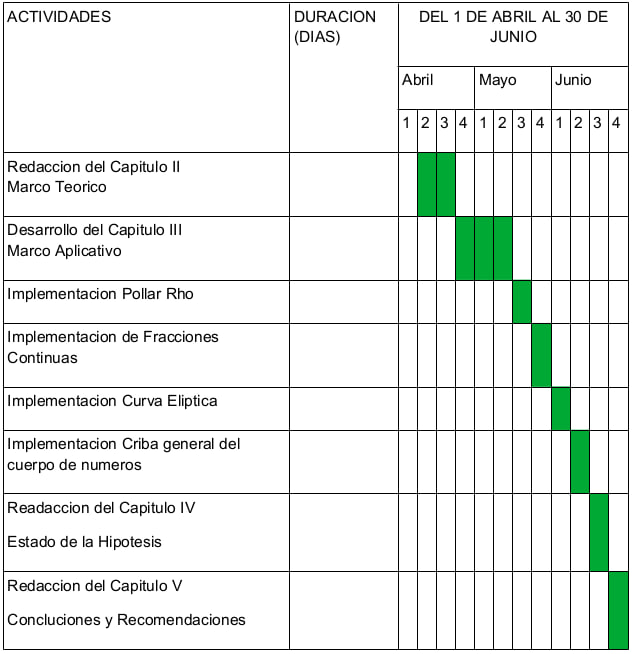
\includegraphics[scale=1]{images/cronograma.jpg}

    \clearpage
    \chapter{INDICE TENTATIVO}
    \begin{enumerate}
        \item{CAPITULO 1 INTRODUCCION}
        \begin{enumerate}
            \item{ANTECEDENTES}
            \item{PLANTEAMIENTO DEL PROBLEMA}
            \item{OBJETIVOS}
            \begin{enumerate}
                \item{OBJETIVO GENERAL}
                \item{OBJETIVOS ESPECIFICOS}
            \end{enumerate}
            \item{JUSTIFICACION}
            \item{ALCANCES Y LIMITES}
            \item{METODOLOGIA}
        \end{enumerate}
        \item{CAPITULO II MARCO TEORICO}
        \begin{enumerate}
            \item{FACTORIZACION DE NUMEROS ENTEROS}
            \item{METODOS DE FACTORIZACION DE NUMEROS ENTEROS}
            \item{ANALISIS DE COMPLEJIDAD DE ALGORITMOS DE FACTORIZACION DE NUMEROS ENTEROS}
        \end{enumerate}
        \item{CAPITULO III MARCO APLICATIVO}
        \begin{enumerate}
            \item{IMPLEMENTACION DEL ALGORITMO 1}
            \item{IMPLEMENTACION DEL ALGORITMO 2}
            \item{IMPLEMENTACION DEL ALGORITMO 3}
            \item{IMPLEMENTACION DEL ALGORITMO 4}
            \item{IMPLEMENTACION DEL ALGORITMO 5}
        \end{enumerate}
        \item{CAPITULO IV RESULTADOS Y ANALISIS}
        \item{CAPITULO V CONCLUCIONES Y RECOMENDACIONES}
        \item{BIBLIOGRAFIA}
        \item{ANEXOS}
    \end{enumerate}

    \chapter{BIBLIOGRAFIA}
    \begin{itemize}
        \item{Abiodun E. Adeyemi, 2019, On Odd Perfect, MultiPerfect and Harmonic Number [en linea], Department of Mathematics University of Ibadan,<https://arxiv.org/pdf/1906.05798.pdf> [13 de junio de 2019]}
        \item{KAM HUNG YAU, 2019, REPRESENTATION OF AN INTEGER AS THE SUM OF A PRIME IN ARITHMETIC PROGRESSION AND A SQUARE-FREE INTEGER WITH PARITY ON THE NUMBER OF PRIME FACTORS [en linea],<https://arxiv.org/pdf/1904.06783.pdf>[13 de junio de 2019]}
    \end{itemize}
    
    \chapter{ANEXOS}
    \section{ANEXO A - ARBOL de PROBLEMA}
    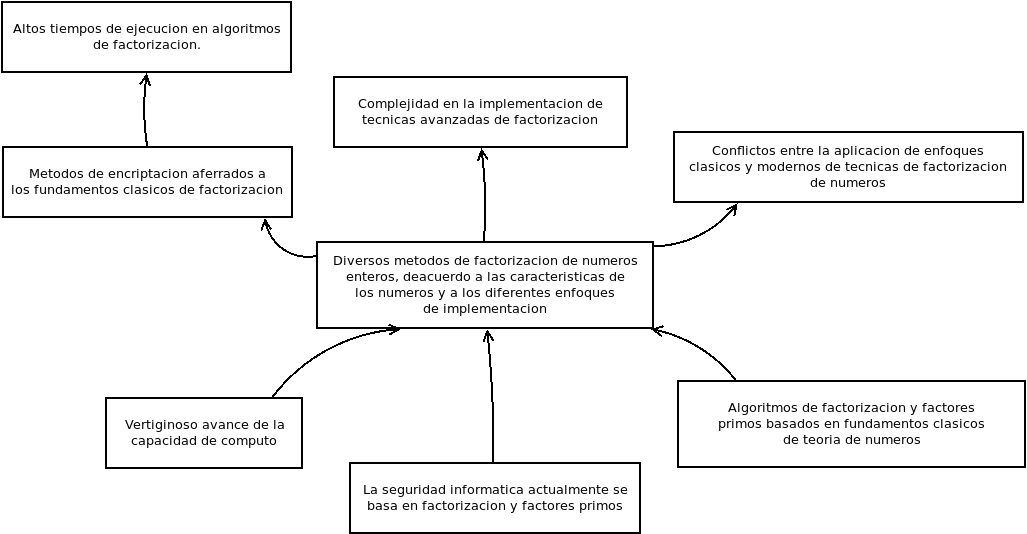
\includegraphics[scale=0.5]{images/arbol_problemas.png}


    % %\input{capitulos/11-indice-tentativo}
    
    % %\input{capitulos/12-cronograma-de-avance}

    % \input{capitulos/III/index}
    
    % \input{capitulos/13-bibliografia}

    % \input{capitulos/03-anexos}
        
    %\input{capitulos/anexos}
    % \endgroup
    % \bibliographystyle{apacite}
    % \bibliography{capitulos/biblio.bib}
	%--------------------------------------------------
	
	
	
	%BACKMATTER
	%---------------------------------------------------
% 	\backmatter
% 	%BIBLIOGRAFÍA.
% 	%\cleardoublepage
% 	\addcontentsline{toc}{chapter}{Bibliografía}
% 	\bibliographystyle{apalike}
% 		\bibliography{capitulos/biblio}
		
	%---------------------------------------------------	
	
\end{document}


%NO OLVIDAR CITAR!